\section{ETA: Early Network Telemetry Flow Analyzer Approach}
%apf eta 

In this section, we first define the model used by our proposed approach to decide whether or not network telemetry data is sent to an INT collector. Then, we describe how it is implemented in a SmartNIC and discuss existing limitations and challenges.

\subsection{Model and Problem Definition}

We consider that a programmable forwarding device $d \in D$ has $N \in \mathbb{N}^{+}$ available metadata to be collected by an INT-enabled packet $p$ and that such packet has a limited available capacity to carry up to $M \in \mathbb{N}^{+}$ of such $N$ items ($M \geq N$). For simplicity, we assume that all devices $D$ have the same telemetry information and that an INT-enabled packet $p$ can only collect telemetry data atomically, that is, it either collects all $N$ metadata from $d \in D$ or none of them. Packet $p$ can only collect once the same subset of telemetry data from the device $d$. We assume that the INT source instructs the packet $p$ correctly according to a given algorithm (e.g., \cite{JISA2019-int}). 

Consider that a packet $p$ has collected $M' \subseteq M$ telemetry data along its routing path -- which comprises a subset of $D$ devices. When the packet $p$ gets to the INT sink node, the question to be answered is: \textit{should it be sent to the INT collector or not?} To answer this question, the INT sink node computes (i) a weighted average of metadata $M'$ collected by packet $p$ and (ii) an exponential weighted moving average. The former tends to weigh the collected telemetry data differently according to its importance. For instance, the processing time (or the queue utilization) metadata might be more important to be considered in the decision process than the packet size. In turn, the latter tends to keep in memory the observed behavior of the latest received telemetry information over time. 

Upon a received packet $p$ in the INT sink node, it extracts the $M'$ collected telemetry metadata and computes a weighted average per packet $A_p = \sum_{i = 1}^{M^{'}} w_i \cdot M_i$ (Eq. 1), where $w_i \in [0, 1]$ is the i-\textit{th} weight given to the telemetry data. We further assume that $\sum_{i = 1}^{M} w_i = 1$ and that $M_i$ corresponds to the i-\textit{th} collected data. Such individual averages $A_p$ are then summing up into a accumulated weighted average metric within a given time window $W$ (we discuss this design choice next). The time window $W$ is  defined for simplicity as a predefined number of packets. However, it can be extended to other metrics such as a time interval. 

Then, the accumulated weighted average of a given window $W$ is given by $A_w = \frac{\sum_{p = 1}^{W} A_p}{W}$ (Eq. 2). Similarly, the exponential weighted moving average is obtained by $A_e = \alpha \cdot A_w + (1 - \alpha) \cdot A_e$ (Eq. 3) where $\alpha \in [0,1]$ comprises the importance given by the elements obtained in the last window $W$ versus the historical knowledge maintained by the moving average $A_e$. Observe that higher values assigned to $\alpha$ prioritize the behavior on the latest window, while lower values prioritize the observed behavior over time. The decision-making process is made in a per-packet manner; however, the decision-making metrics (e.g., $A_e$) are updated in a time-window manner.


\subsection{Design and Implementation in a SmartNIC}


Figure~\ref{fig-overview} illustrates an overview of the proposed approach pipeline implementation. Our approach utilizes the reference V1Model architecture to programmable forwarding devices as the basis to implement/add such functionalities into the Netronome SmartNIC. Also, our approach is based on P4-16 and in Micro-C languages. 

Upon a packet is received by the SmartNIC, the packet is parsed accordingly. Our approach implementation resides just after the parsing step and the ingress pipeline (where the routing decision takes place), that is, in the egress pipeline. For this discussion, we assume that our forwarding device can process Ethernet frames and IP packets (or any known INT encapsulation protocol). Therefore, we omit the parsing steps since it is trivial and out of this work's scope. We then focused on the following up steps.   

\begin{figure}[t]
\centering
        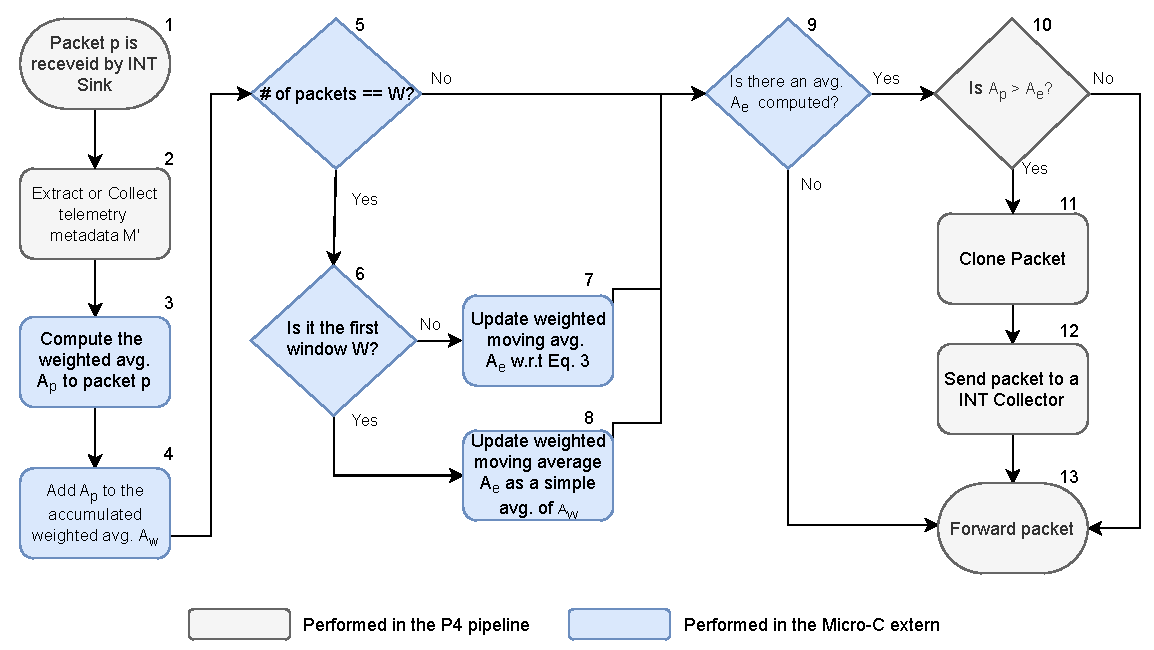
\includegraphics[scale=0.45]{aina-img/apf-overview.pdf}
        \caption{Overview of the proposed P4+Micro-C pipeline approach.}
        \label{fig-overview}
\end{figure}

Our approach is implemented in the INT sink. Therefore, at this stage, all INT telemetry metadata has already been collected. The first steps of our approach consist of receiving the packet and extracting the telemetry data from it -- or, in some cases, collecting them directly from the data plane (this might happen when the INT sink node acts as an INT transit node as well). This corresponds to steps 1 and 2 in Figure~\ref{fig-overview}. The extracted data is then stored in a custom-made metadata header structure -- named \texttt{ETA} metadata struct. This structure comprises $M$ 32-bit structures and a 2-bit flag used to instruct the decision-making process. For instance, if a packet needs to be sent to the INT collector, this flag is used internally. In the Netronome architecture, the existing timestamps (\texttt{ingress\_timestamp} and \texttt{current\_timestamp}) are 48-bit words. However, most of the applications use only the least significant bits (the last 32 bits) since they account for nanosecond differences. Further, as discussed next, the Netronome architecture also limits the results of arithmetic operations to 32 bits words (and therefore, we cannot operate on 48-bits timestamps). After extracting telemetry data into the \texttt{ETA} struct, our implementation calls a Micro-C extern code to handle more complex operations inside the data plane (depicted in Figue~\ref{fig-overview-microc}). For instance, floating-point operations are not allowed in the P4-16 language reference, nor does the SmartNIC natively implement it. To allow the SmartNIC code to be partially written in P4 and Micro-C -- and more importantly, to exchange data between them -- we rely on \texttt{ETA} structs and internal P4 metadata to enable such real-time communications.

%
The Micro-C code starts receiving data from the P4 pipeline and locking up memory regions using a mutex (steps 1-3 in Figue~\ref{fig-overview-microc}). That is necessary since our application shares memory regions between processors/threads to store the current window $W'$, as well as the current values of calculated averages (i.e. $A_e$ and $A_w$). 
%
Next, we calculate $A_p$  and $A_w$ according to Equation 1 and Equation 2, respectively. Figure~\ref{fig-overview-microc} illustrates these procedures in steps 4-7.  It is important to mention that neither the P4 reference architecture nor the Netronome support floating-point instructions. We implemented all these operations using fixed-point representation with 32 bits to surpass that limitation. In short, a fixed-point representation handles all real numbers as integers. The process scales up the numbers by multiplying by a constant factor $C$ and then performs the multiplications/division as a regular integer. Finally, the scaled-up result is scaled down appropriately. In our implementation, we have used a constant $C$ of 16 bits and performed the scale-up operation by applying a bit-shifting operation (i.e., $M'_i << 16$). After calculating $A_p$, we verify whether it is the case to send it out to the INT collector. We compare $A_p$ with the observed $A_e$ (which captures the historical behavior). In case the  $A_p$ packet value is higher than the dynamic $A_e$ one, we mark the packet to be sent out to the collector (steps 8-12 in Figure~\ref{fig-overview-microc}).


As previously mentioned, our approach performs per-packet decisions. However, we update the exponential weighted moving average $A_e$ at the end of a given window $W$. This is done because the average $A_e$ depends on $A_w$ -- and, the Netronome architecture does not allow arbitrary integer divisions (only by the power of 2 by performing bit-shifting -- for instance $M'_i >> 16$). Our approach verifies whether it reaches or not the end of a given window $W$ (step 14 in Figure~\ref{fig-overview-microc}). If so, then it updates the moving average $A_e$ (step 15-19 in Figure~\ref{fig-overview-microc}) according to Equation~3. Further, if it is the first time to reach the window $W$ (i.e., $W' == W$), then $A_e$ assumes a simple average of $A_w$ (step 20 in Figure~\ref{fig-overview-microc}). Then, the Micro-C sets the mutex down and allows other threads to use the blocked shared memory. Last, our Micro-C code returns the calculated values to the original P4 pipeline (step 22-23 in Figure~\ref{fig-overview-microc}). 

\begin{figure}[t]
\centering
        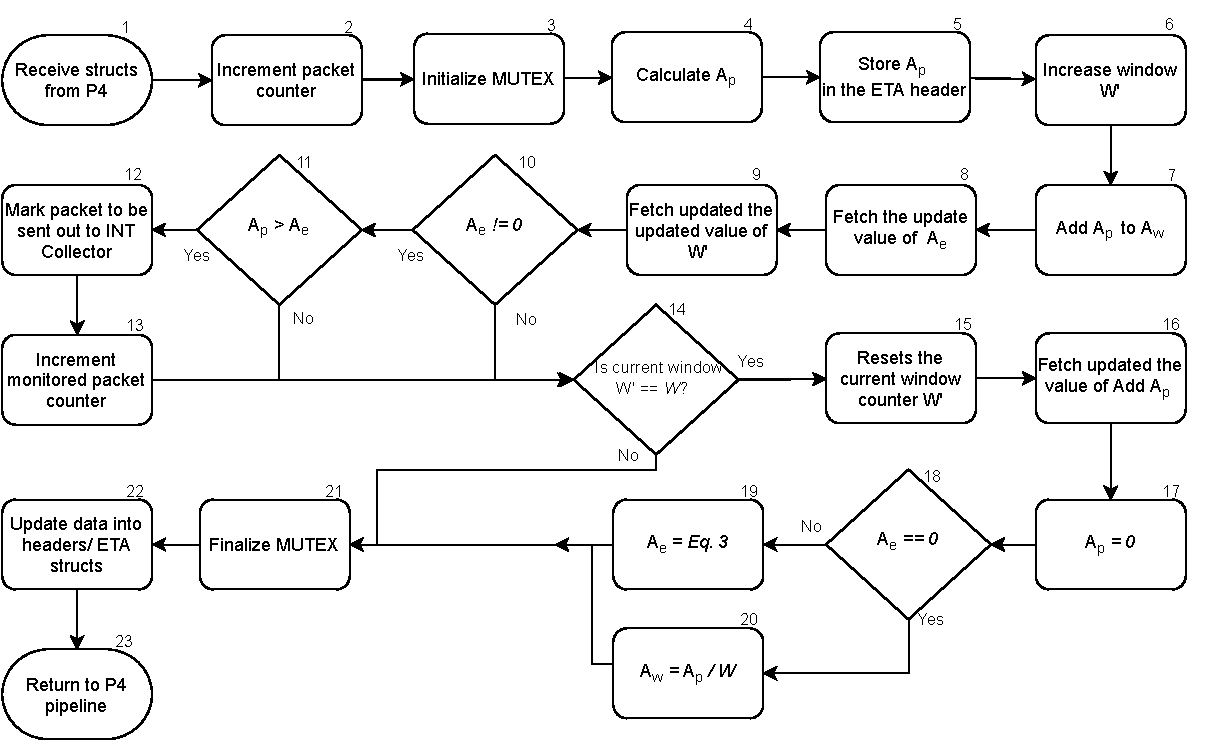
\includegraphics[scale=0.4]{aina-img/apf_micro_c.pdf}
        \caption{Overview of the proposed Micro-C routine.}
        \label{fig-overview-microc}
\end{figure}

Back in the P4 pipeline (Figure~\ref{fig-overview}), our approach clone and recirculate the packet $p$. The original packet is forwarded to its destination (step 13 in Figure~\ref{fig-overview}), while the cloned one is sent to the INT collector (step 12 in Figure~\ref{fig-overview}).

%To send the information back to the P4 pipeline, we use the same \texttt{ETA} struct as an auxiliary variable to store partial results (e.g.,  $A_p$). Then, we add $A_p$ to the partial sum of $A_w$, which will be calculated at the end of window $W$. The reason behind adopting this window strategy is because the Netronome Architecture does not support arbitrary division operations. In fact, it only supports division by a multiple of a power of 2.

%Then, we verify if our current window counting reaches the window size $W$. If so, it means that we need to calculate (in case it is the first) or recalculate our $A_e$ according to Equation 3. 


%\begin{figure}[t]
%\centering
%        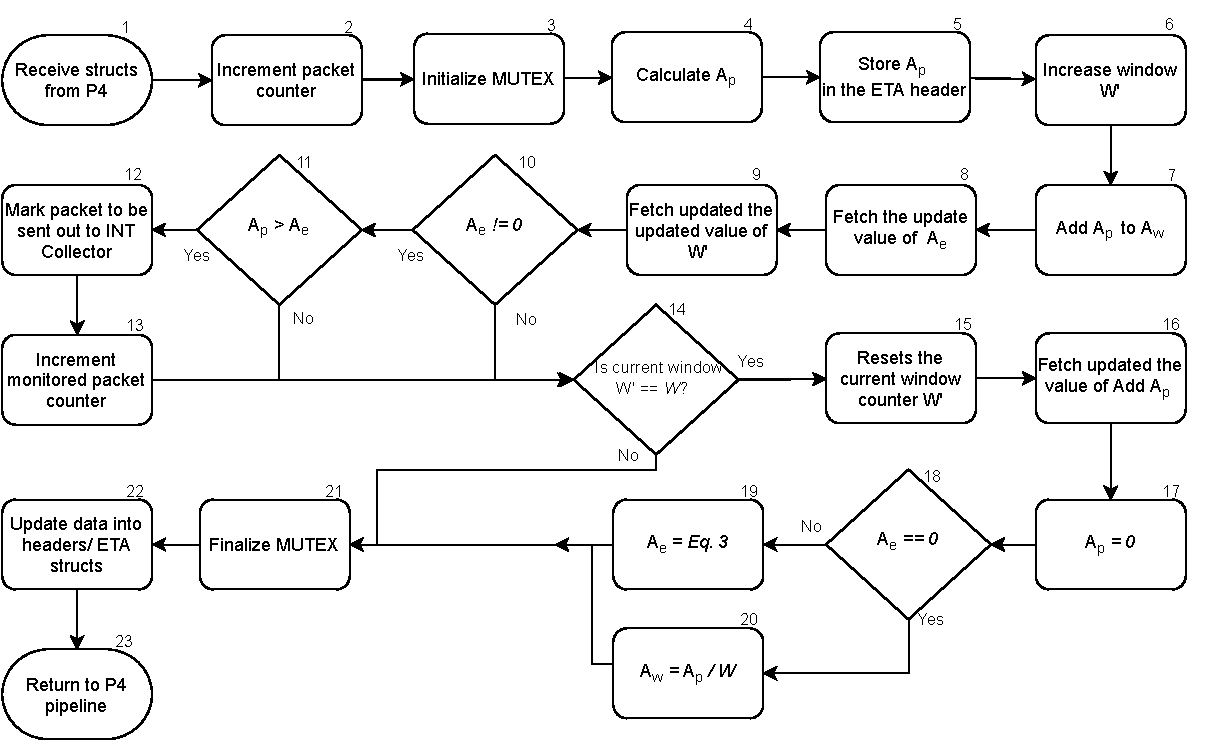
\includegraphics[scale=0.55]{aina-img/apf_micro_c.pdf}
%        \caption{Overview of the proposed Micro-C approach.}
%        \label{fig-overview-microc}
%\end{figure}

%\subsection{Current Limitations of SmartNICs}

%Floating-point operations
%bit-shifting
%registers
%control-based structes
%metadata